\subsection{Interface}
    These are the commands that the web API will be using to maintain the database and receive commands.

    \subsubsection{AuthenticateAdmin}
        Checks the inputted password against the listed valid password to allow website use.
        \begin{itemize}
            \item Headers required:
            \begin{itemize}
                 \item none
             \end{itemize}
            \item POST arguments:
            \begin{itemize}
                 \item password : String
             \end{itemize}
             \item Statuses:
            \begin{itemize}
                \item 200 OK:
                \begin{itemize}
                    \item boolean : true/false
                \end{itemize}
                \item 400 Bad Request
                \item 500 Internal Server Error
            \end{itemize}
       \end{itemize}

    \subsubsection{AddRecord}
        Adds a record to the database, and returns the record ID. Used by the Android application.
        \begin{itemize}
            \item Headers required:
            \begin{itemize}
                \item none
            \end{itemize}
            \item POST arguments:
            \begin{itemize}
                \item record : Record
            \end{itemize}
            \item Statuses:
            \begin{itemize}
                \item 200 OK:
                \begin{itemize}
                    \item record ID : Integer
                \end{itemize}
                \item 400 Bad Request
                \item 500 Internal Server Error
             \end{itemize}
        \end{itemize}

    \subsubsection{AddReserve}
        Adds a reserve to the database, and returns the reserve ID.
        \begin{itemize}
            \item Headers required:
            \begin{itemize}
                \item none
            \end{itemize}
            \item POST arguments:
            \begin{itemize}
                \item reserve : Reserve
            \end{itemize}
            \item Statuses:
            \begin{itemize}
                \item 200 OK:
                \begin{itemize}
                    \item reserve ID : Integer
                \end{itemize}
                \item 400 Bad Request
                \item 500 Internal Server Error
            \end{itemize}
        \end{itemize}
    

    \subsubsection{RemoveSpecimen}
        Removes a single specimen from the database, provided an ID and an administrator password. Used by the web site.
        \begin{itemize}
            \item Headers required: 
            \begin{itemize}
                \item none
            \end{itemize}
            \item POST Arguments:
            \begin{itemize}
                \item specimenID : Integer
                \item password : String
            \end{itemize}
            \item Statuses:
            \begin{itemize}
                \item 200 OK : no data
                \item 400 Bad Request
                \item 401 Unauthorized
                \item 500 Internal Server Error
            \end{itemize}
        \end{itemize}


    \subsubsection{GetSpecimen}
        Returns a single specimen result, which includes data from the record the specimen belongs to when provided an ID. Used by the web site.
        \begin{itemize}
            \item Headers required: 
            \begin{itemize}
                \item none
            \end{itemize}
            \item POST Arguments:
            \begin{itemize}
                \item specimenID : Integer
            \end{itemize}
            \item Statuses:
            \begin{itemize}
                \item 200 OK :
                \begin{itemize}
                    \item specimen : SpecimenResult
                \end{itemize}
                \item 400 Bad Request
                \item 500 Internal Server Error
            \end{itemize}
        \end{itemize}


    \subsubsection{UpdateSpecimen}
        Updates a specific Specimen by ID.
        \begin{itemize}
            \item Headers Required:
            \begin{itemize}
                \item none
            \end{itemize}
            \item POST Arguments:
            \begin{itemize}
                \item specimenID : int
                \item password : String
            \end{itemize}
            \item Statuses: 
            \begin{itemize}
                \item 200 OK :
                \item 400 Bad Request
                \item 500 Internal Server Error
            \end{itemize}
        \end{itemize}

    \subsubitem{GetSpecimens}
        Returns a list of specimen results, which include data from the record the specimen belongs to, searching and sorting them by defined criteria. Used by the web site.
        \begin{itemize}
            \item Headers Required:
            \begin{itemize}
                \item none
            \end{itemize}
            \item POST Arguments:
            \begin{itemize}
                \item order : String (``ascending'' or ``descending'')
                \item method : String (``speciesName'', ``locationName'', ``userName'', ``timestamp'')
                \item value : String
                \item column : String (``speciesName'', ``locationName'', ``userName'')
            \end{itemize}
            \item Statuses: 
            \begin{itemize}
                \item 200 OK : array of SpecimenResult
                \item 400 Bad Request
                \item 500 Internal Server Error
            \end{itemize}
        \end{itemize}

    \subsubsection{AddResource}
        Adds a file resource to the server, and returns an ID. Used by the Android application and the web site.
        \begin{itemize}
            \item Headers required: 
            \begin{itemize}
                \item none
            \end{itemize}
            \item POST Arguments:
            \begin{itemize}
                \item resource : OctetStream
            \end{itemize}
            \item Statuses:
            \begin{itemize}
                \item 200 OK :
                \begin{itemize}
                    \item resource ID : Integer
                \end{itemize}
                \item 400 Bad Request
                \item 500 Internal Server Error
            \end{itemize}
        \end{itemize}

    \subsubsection{GetResource}
        Returns a file resource when provided with a resource ID. Used by the web site.
        \begin{itemize}
            \item Headers required:
            \begin{itemize}
                \item none
            \end{itemize}
            \item POST Arguments:
            \begin{itemize}
                \item resourceID : Integer
            \end{itemize}
            \item Statuses:
            \begin{itemize}
                \item 200 OK : 
                \begin{itemize}
                    \item resource data : OctetStream
                \end{itemize}
                \item 400 Bad Request
                \item 500 Internal Server Error
            \end{itemize}
        \end{itemize}

    \subsubsection{GetReserve}
        Returns a single reserve result, which holds data about a location used by records. 
        \begin{itemize}
            \item Headers required: 
            \begin{itemize}
                \item none
            \end{itemize}
            \item POST Arguments:
            \begin{itemize}
                \item reserveID : Integer
            \end{itemize}
            \item Statuses:
            \begin{itemize}
                \item 200 OK :
                \begin{itemize}
                    \item reserve : Reserve
                \end{itemize}
                \item 400 Bad Request
                \item 500 Internal Server Error
            \end{itemize}
        \end{itemize}       

    \subsubsection{GetReserves}
        Returns a list of distinct locations used by records in the database for use by the Android application.
        \begin{itemize}
            \item Headers Required:
            \begin{itemize}
                    \item none
            \end{itemize}
            \item POST Arguments:
            \begin{itemize}
                    \item none
            \end{itemize}
            \item Statuses: 
            \begin{itemize}
                    \item 200 OK : array of Reserve
                    \item 400 Bad Request
                    \item 500 Internal Server Error
            \end{itemize}
        \end{itemize}


    \subsubsection{UpdateReserve}
        Updates a specific Reserve by ID.
        \begin{itemize}
            \item Headers Required:
            \begin{itemize}
                \item none
                \end{itemize}
                \item POST Arguments:
                \begin{itemize}
                        \item reserveID : int
                \item password : String
            \end{itemize}
            \item Statuses: 
            \begin{itemize}
                    \item 200 OK :
                    \item 400 Bad Request
                    \item 500 Internal Server Error
            \end{itemize}
        \end{itemize}


    \subsubsection{RemoveReserve}
        Removes a specific Reserve by ID.
        \begin{itemize}
            \item Headers Required:
            \begin{itemize}
                \item none
            \end{itemize}
            \item POST Arguments:
            \begin{itemize}
                \item reserveID : int
                \item password : String
            \end{itemize}
            \item Statuses: 
            \begin{itemize}
                \item 200 OK : 
                \item 400 Bad Request
                \item 500 Internal Server Error
            \end{itemize}
        \end{itemize}


\subsection{Detailed design}
    \subsubsection{Diagrams}
        \begin{figure}
            \centering
            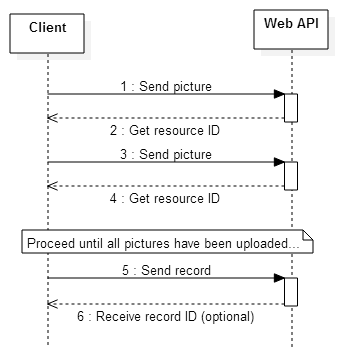
\includegraphics[scale=0.75]{server/working/SequenceDiagram-AddRecord.png}
            \caption{Sequence diagram: adding a record through the web API}
            \label{fig:addRecordSequenceDiagram}
        \end{figure}

        \begin{landscape}
            \begin{figure}
                \centering
                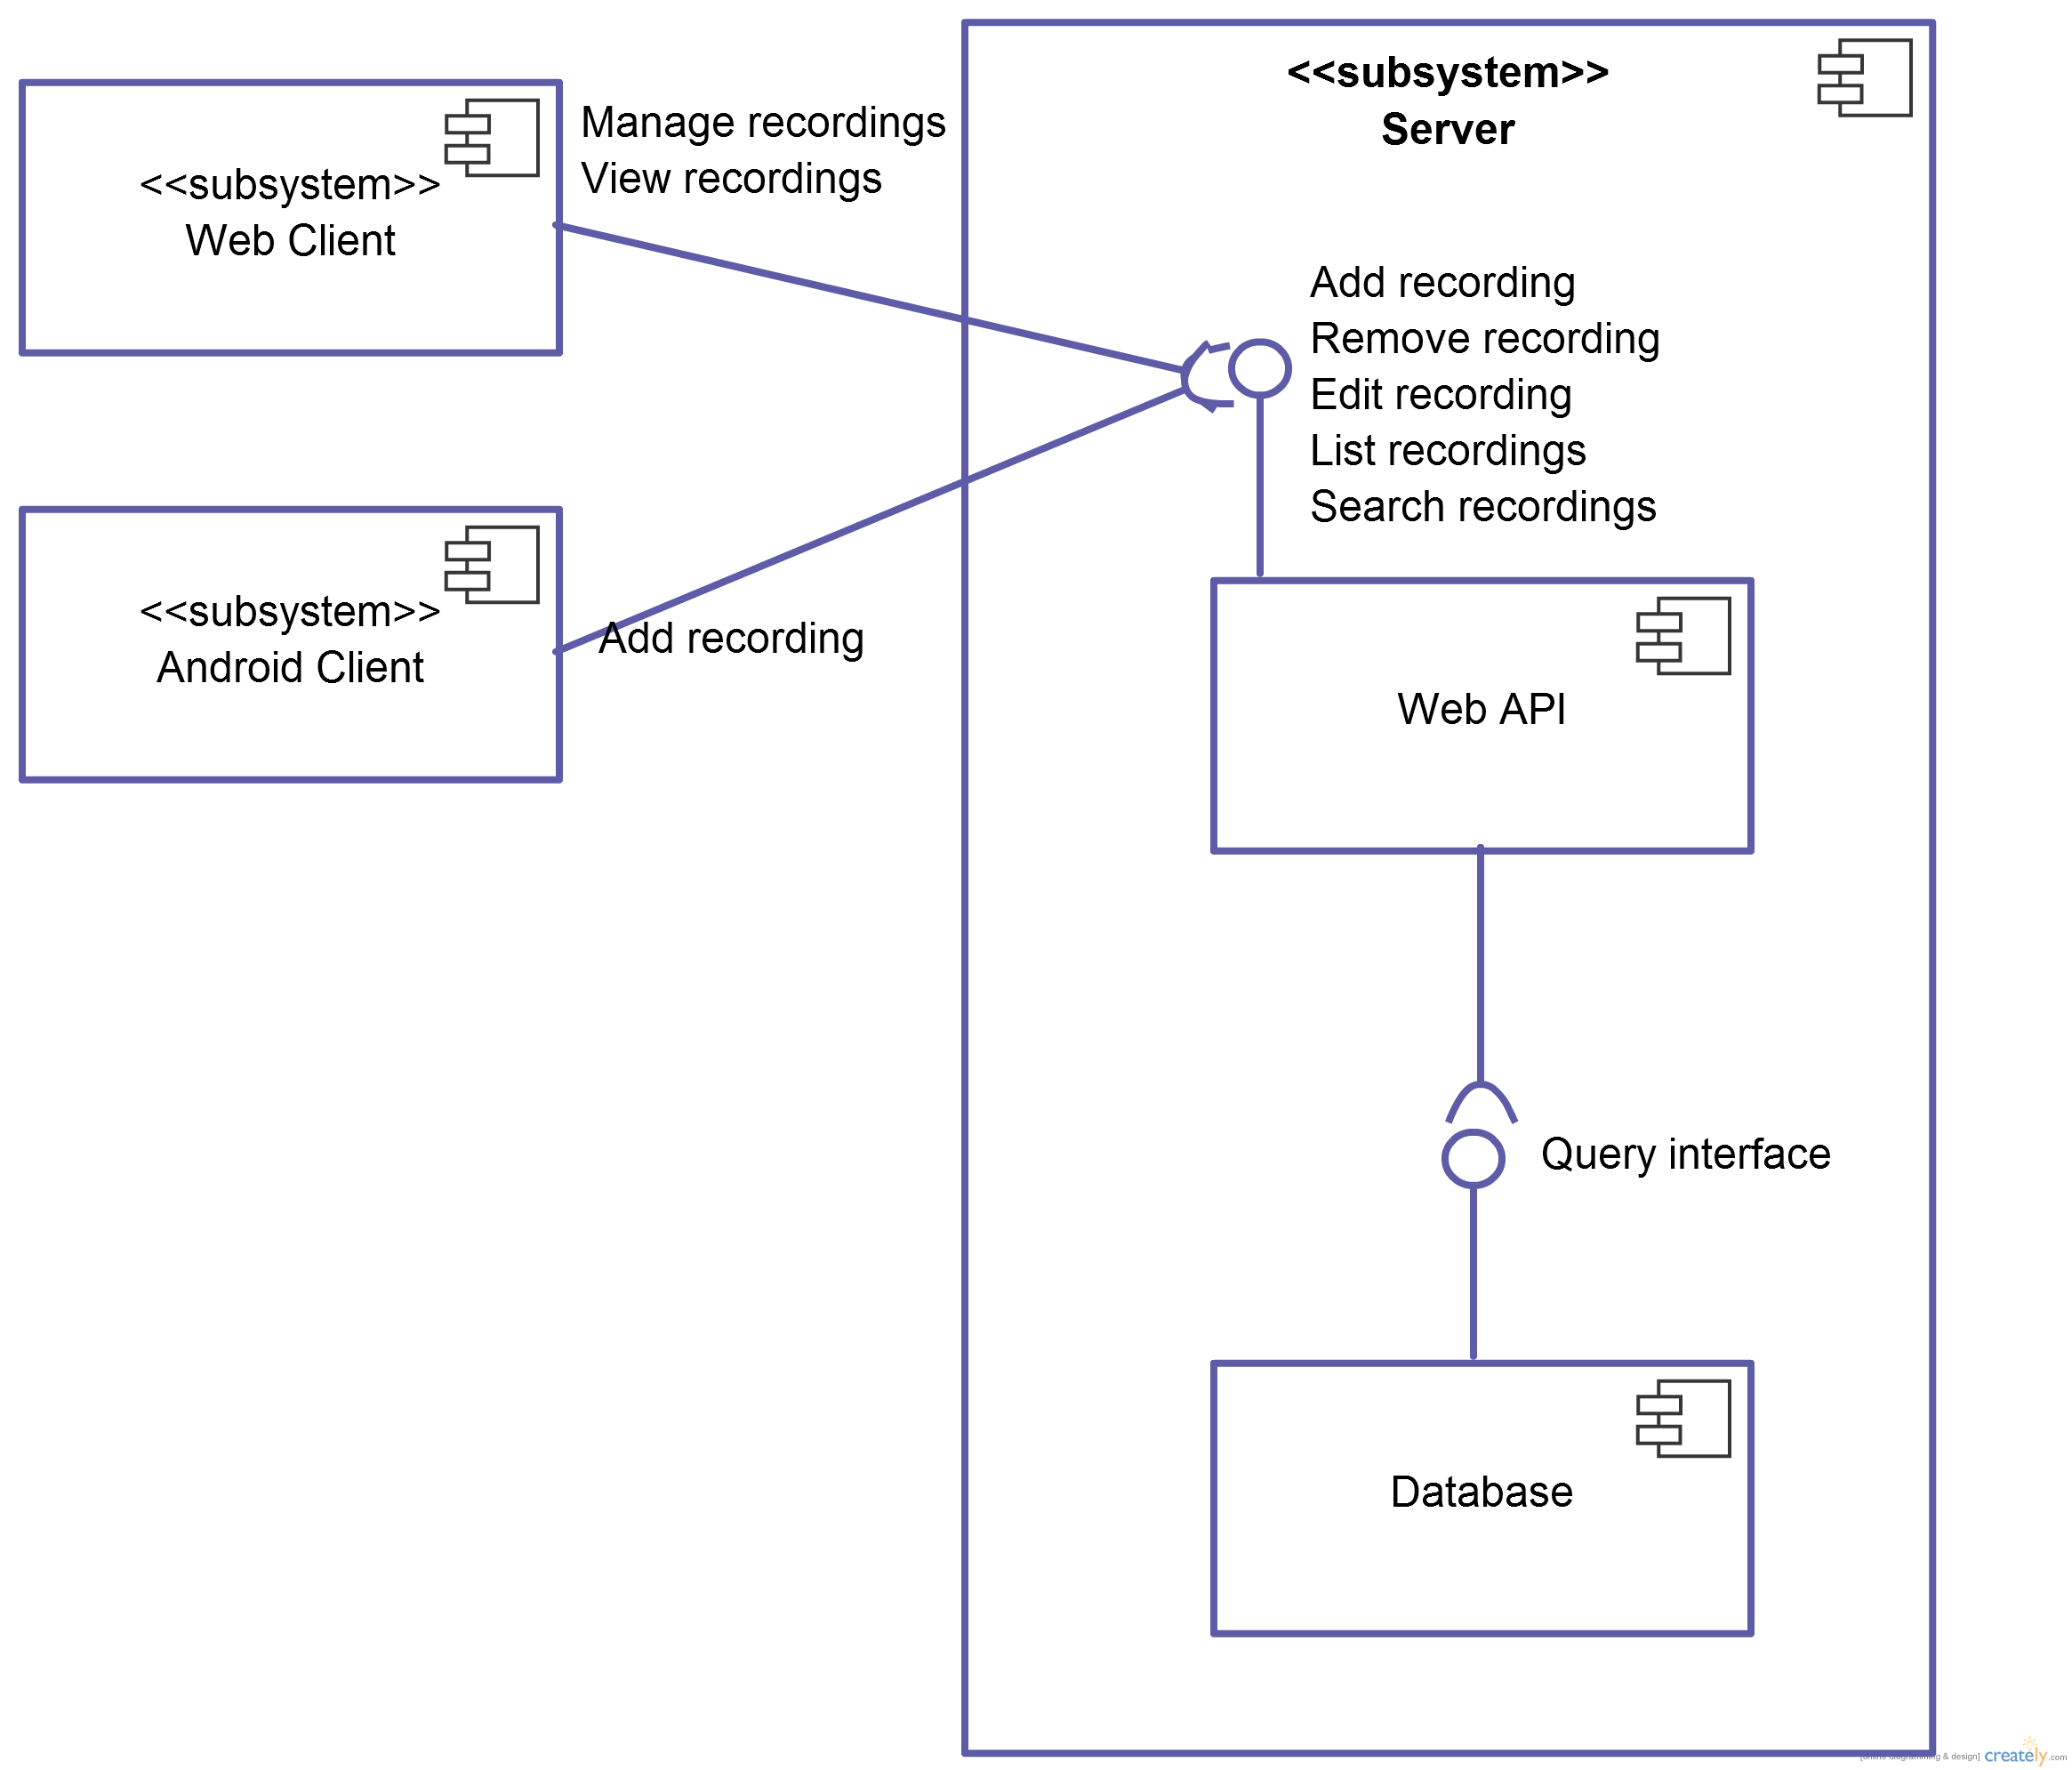
\includegraphics[scale=0.2]{server/ComponentDiagram.png}
                \caption{Web Api component Diagram}
                \label{fig:webAPIComponentDiagram}
            \end{figure}
        \end{landscape}

    \subsubsection{Significant data structures}

        The web API is going to make use of the Record, Specimen, RecordLocation and SpecimenResult data structures, which will be exchanged between the server and its clients (the Android application and the website). They will be represented in a JSON format, which is readily available for use in PHP, JavaScript, and Android. Data types, where specified, are JSON data types. 

        The structure of a Record is as follows:
        \begin{itemize}
            \item Record : Object
            \begin{itemize}
                \item UserName : String
                \item UserPhone : String
                \item UserEmail : String
                \item LocationName : String 
                \item Timestamp : Number 
                \item LocationOS : String
                \item Specimens : Array of Specimen
            \end{itemize}
        \end{itemize}
        
        The structure of a Reserve is as follows:
        \begin{itemize}
            \item Reserve : Object
            \begin{itemize}
                \item ReserveID : Number
                \item LocationName : String 
                \item LocationOS : String
                \item Description : String
            \end{itemize}
        \end{itemize}

        The structure of a Specimen is as follows:
        \begin{itemize}
            \item Specimen : Object
            \begin{itemize}
                \item SpeciesName : String
                \item LocationLatitude : Number
                \item LocationLongtitude : Number
                \item Abundance : Number
                \item Comment : String
                \item ScenePhoto : String (ID of a resource on the server)
                \item SpecimenPhoto : String (ID of a resource on the server)
            \end{itemize}
        \end{itemize}
        
        The structure of a SpecimenResult is as follows:
        \begin{itemize}
            \item SpecimenResult : Object
            \begin{itemize}
                \item UserID : Number
                \item RecordID : Number
                \item SpecimenID : Number
                \item UserName : String
                \item UserEmail : String
                \item UserPhone : String
                \item LocationName : String
                \item LocationOS : String
                \item Timestamp : Number
                \item SpeciesName : String
                \item LocationLatitude : Number
                \item LocationLongtitude : Number
                \item Abundance : Number
                \item Comment : String
                \item ScenePhoto : String (ID of a resource on the server)
                \item SpecimenPhoto : String (ID of a resource on the server)
            \end{itemize}
        \end{itemize}

        The web API uses config.php as a configuration store. It contains the \$CONFIG array, containing the following entries:
        
         \begin{itemize}
                \item dbname : the address of the MySQL database to be used
                \item username : the user name to use on the MySQL database
                \item password : the password to use on the MySQL database
                \item adminPassword : the password used in the DeleteSpecimen web method
        \end{itemize}
        The web API is going to use a relational database as a data store.
        The database tables are as follows:

        \begin{itemize}
            \item Users
            \begin{itemize}
                \item UserId : INT auto-increment PK
                \item UserName : VARCHAR(20) not-null
                \item UserFullName : VARCHAR(50)
                \item UserPhone : VARCHAR(20)
                \item UserEmail : VARCHAR(50)
                \item UserPassword : BINARY(20)
            \end{itemize}
                
            \item Records
            \begin{itemize}
                \item RecordId : INT auto-increment PK
                \item UserId : INT not-null
                \item LocationName : VARCHAR(50)
                \item Timestamp : INT
                \item LocationOS : VARCHAR(10)
            \end{itemize}
                
            \item Resources
            \begin{itemize}
                \item ResourceId : INT auto-increment PK
            \end{itemize}
            
            \item Reserves
            \begin{itemize}
                \item ReserveID : INT auto-increment PK
                \item LocationName : VARCHAR(50)
                \item LocationOS : VARCHAR(10)
                \item Description : TEXT
            \end{itemize}

            \item Specimens
            \begin{itemize}
                \item SpecimenId : INT auto-increment PK
                \item RecordId : INT not-null
                \item SpeciesName : VARCHAR(255) not-null
                \item Latitude : FLOAT(10,6)
                \item Longitude : FLOAT(10,6)
                \item Abundance : INT
                \item Comment : TEXT
                \item ScenePhoto : INT
                \item SpecimenPhoto : INT   
            \end{itemize}
            \end{itemize}